\clearpage
\appendix
\raggedbottom
\renewcommand{\thesection}{Appendix \Alph{section}}
\renewcommand{\thesubsection}{\Alph{section}.\arabic{subsection}}
\setcounter{figure}{0}
\renewcommand{\thefigure}{A\arabic{figure}}
\renewcommand{\theHfigure}{A\arabic{figure}}
\section{Methods and complete per-cell results}

\subsection{Cohorts, models, training and compute}\label{cohorts-models-training-and-compute}

\textbf{Cohorts and eligibility.} Two public datasets supply the three cohorts: VitalDB, and
MOVER, whose single release carries both an EPIC-derived and an SIS-derived arm. Both are de-identified. VitalDB v1.0.0 is openly accessible from PhysioNet under the Creative Commons Attribution 4.0 International (CC BY 4.0) license; MOVER is available from the UCI Machine Learning Repository to researchers who sign its data use agreement. Development
used MOVER's EPIC arm. The subject-aware split at
seed 1004 gave 6,409 training, 1,375 validation and 1,404 test cases
out of 9,188, split on unique subject identifiers so that a patient with several operations
lands in one fold. The test split holds 1,404 cases, 786 with a sustained event, 1,145 subjects.
External evaluation used VitalDB, with 2,804 cases, 1,007 events and 2,730 subjects, and the
SIS-derived arm of MOVER, with 2,641 cases and 1,409 events, neither of which contributed to training, calibration or threshold selection. Neither arm of MOVER carries a subject key that resolves against the other, so that statement holds at the level of the released records and cannot be checked at the level of patients. Per-minute eligibility
drops the induction prefix, 25 minutes where the record is anchored on anesthesia start, 10
where it is anchored on surgical start, and every minute at or after first onset, so no
model is asked to predict an event already in progress. Event cases required five valid
pre-onset minutes after that exclusion and controls thirty. Procedure group is never a model
input in any family: it separates the cohorts almost perfectly and would be learned as cohort
identity.

\textbf{Training samples, labels and the offset used here.} Training uses one sample per case: the
120-minute window ending at that case's reference time, labeled 1 if the case has a sustained
event and 0 otherwise. There is no per-minute training target. For an event case the reference
time is the first sustained-onset minute shifted back by a lead-time offset, and that offset is
\textbf{zero for every model reported in this paper}, so the reference time is onset itself. A control
has no onset, so it is given a sampled pseudo-onset: its onset ratio, onset divided by case
length, is drawn with replacement from the event cases of the same source cohort and multiplied
by the control's own case length, then resampled rather than clipped until it falls inside the
eligible range, so the control reference times match the event distribution within each source.
Event cases with fewer than five eligible pre-onset minutes and controls shorter than thirty are
dropped before that sampling. The scored checkpoint is the epoch with the best validation AUROC,
and it is the only one used. Evaluation departs from training in the one respect that matters
here: every eligible minute of a case is scored independently and inherits its case's label, and
\texttt{t\_\allowbreak{}to\_\allowbreak{}event} is measured against that same reference time, real onset for an event case and the
sampled pseudo-onset for a control.

\textbf{Features.} The same twenty inputs for every family: sixteen per-minute channels, being
MAP, systolic and diastolic pressure, their non-invasive counterparts, heart rate, SpO2,
end-tidal CO2, temperature, FiO2, MAC, tidal volume, respiratory rate, PEEP and peak
inspiratory pressure, and four demographics, being age, sex, height and weight. The families
differ in how they consume them. The transformer takes each non-missing cell as a
(type, time, value) triplet with demographics as a fixed prefix at time zero, up to 2,048
tokens over a 120-minute window, so missing cells produce no token and are never imputed. The
LSTM takes the normalized per-minute window as a value-and-mask pair per channel. Logistic
regression, random forest and XGBoost take the last observation carried forward per channel
plus the demographics. Per-channel median and interquartile scaling was fitted on the
training cases alone and applied unchanged everywhere else.

\textbf{Architectures and training.} Seed 1004 throughout. The transformer is a STraTS-style
encoder, a type embedding plus a value MLP plus a time MLP summed per triplet, two encoder
layers, model width 128, four heads, feed-forward width 512, dropout 0.1, a learnable
classification token and a two-class softmax head; AdamW at learning rate 1.2e-3, weight
decay 1e-2 applied to two-dimensional tensors only, gradient clipping at 1.0, a cosine
schedule with 5\% warmup, batch size 64, cross-entropy, up to 50 epochs with early stopping on
validation AUROC at patience 10, under bfloat16 autocast. The LSTM is one layer of width 128
with dropout 0.1, AdamW at 1e-3 with weight decay 1e-2, batch size 64, up to 40 epochs at
patience 8. Logistic regression is median imputation and standardization followed by an L2
fit at up to 2,000 iterations. The random forest is 400 trees. XGBoost is 600 rounds at depth
6, learning rate 0.05, row and column subsampling at 0.8, histogram tree method, early
stopping after 40 rounds on validation AUC. No hyperparameter search was run over any of
these values.

\textbf{Compute.} Every model was trained on one Apple M3 Ultra desktop with 512 GB of unified
memory, using PyTorch 2.10 on the Metal backend with bfloat16 autocast; no GPU cluster was
used. Wall clock for the five models reported here was 40.3 minutes for the transformer, 14.5
for the LSTM, 3.6 for the random forest, and 34 and 33 seconds for XGBoost and logistic
regression. The project trained more than this paper reports: each family was also trained at
seven lead-time offsets, of which the transformer arm alone took 3.8 hours. The analyses in
this paper add no training and read cached per-minute scores on the same machine. Software
was PyTorch 2.10.0, scikit-learn 1.7.1, XGBoost 3.3.0, NumPy
2.2.6, pandas 2.3.2 and SciPy 1.16.1.

\textbf{Data and code.} Both source datasets are public and de-identified. VitalDB v1.0.0 is openly accessible from PhysioNet under the Creative Commons Attribution 4.0 International (CC BY 4.0) license; MOVER is available from the UCI Machine Learning Repository under its data use agreement, one download supplying both arms used here. An
institutional review board granted this secondary analysis an exemption from review and a
waiver of consent, its identity and protocol number withheld for anonymous review. This work
added no data collection and no patient contact. Analysis code is available at an anonymized repository,
\url{https://anonymous.4open.science/r/ioh-leadtime-anon-BD0E}, under the Apache License 2.0.
The repository carries the analysis code and the aggregate result files behind the tables and figures, and no patient-level or derived patient-level data of any kind; each dataset is obtained from its own provider under the access and license terms above.

\subsection{Lead time by quantile-derived band of observed window, all fifteen cells}\label{lead-time-by-quantile-derived-band-of-observed-window-all-fifteen-cells}

\begin{minipage}{\linewidth}
\textbf{Table A1 \textbar{} Median alert lead time by quantile-derived band of observed window, all fifteen
cells.} Main text Section 3.1 reports the ITE Transformer. The gradient is positive in
every cell.
\texttt{Bands} is the number of quantile-derived groups actually realized: where the observed window is censored
at the 60-minute alert window the upper quintiles collapse onto a single value, and
duplicate edges are dropped rather than bands invented.
The gradient is the difference of the highest and lowest band medians, and its interval is the
paired cluster bootstrap of that difference: one weight matrix is drawn per cell and reused
across bands, and the band edges and the window span are held fixed at their full-sample values
so the ratio's denominator is not itself resampled. The interval excludes zero in all fifteen
cells. \texttt{Lead\ min\ per\ window\ min} is the ratio of those two between-band median contrasts and not
a per-case slope, so a value slightly above 1.0 carries no contradiction with the per-case
constraint that a lead cannot exceed its own window.

\vspace{0.5em}
\centering\footnotesize
\begin{tabular}{@{}
  >{\raggedright\arraybackslash}p{(\columnwidth - 12\tabcolsep) * \real{0.14}}
  >{\raggedright\arraybackslash}p{(\columnwidth - 12\tabcolsep) * \real{0.14}}
  >{\raggedleft\arraybackslash}p{(\columnwidth - 12\tabcolsep) * \real{0.18}}
  >{\raggedright\arraybackslash}p{(\columnwidth - 12\tabcolsep) * \real{0.14}}
  >{\raggedright\arraybackslash}p{(\columnwidth - 12\tabcolsep) * \real{0.14}}
  >{\raggedright\arraybackslash}p{(\columnwidth - 12\tabcolsep) * \real{0.14}}
  >{\raggedright\arraybackslash}p{(\columnwidth - 12\tabcolsep) * \real{0.14}}@{}}
\toprule
Model & Cohort & Bands & Window Q1$\rightarrow$last, min & Lead Q1$\rightarrow$last, min & Gradient, min (95\% CI) & Lead min per window min (95\% CI) \\
\midrule
Transformer & MOVER (EPIC) test & 4 & 10 $\rightarrow$ 60 & 9 $\rightarrow$ 46 & +37 {[}+35, +41{]} & 0.74 {[}0.70, 0.82{]} \\
Transformer & VitalDB & 5 & 7 $\rightarrow$ 60 & 5 $\rightarrow$ 59 & +54 {[}+51, +55{]} & 1.02 {[}0.96, 1.04{]} \\
Transformer & MOVER (SIS) & 4 & 8 $\rightarrow$ 60 & 6 $\rightarrow$ 46 & +40 {[}+37, +43{]} & 0.77 {[}0.71, 0.83{]} \\
LSTM & MOVER (EPIC) test & 4 & 10 $\rightarrow$ 60 & 6 $\rightarrow$ 44 & +38 {[}+35, +41{]} & 0.77 {[}0.70, 0.82{]} \\
LSTM & VitalDB & 5 & 6 $\rightarrow$ 60 & 3 $\rightarrow$ 34 & +31 {[}+21, +48{]} & 0.57 {[}0.39, 0.89{]} \\
LSTM & MOVER (SIS) & 4 & 9 $\rightarrow$ 60 & 5 $\rightarrow$ 31 & +26 {[}+19, +30{]} & 0.51 {[}0.37, 0.59{]} \\
XGBoost & MOVER (EPIC) test & 3 & 12 $\rightarrow$ 60 & 8 $\rightarrow$ 38 & +30 {[}+26, +34{]} & 0.62 {[}0.54, 0.71{]} \\
XGBoost & VitalDB & 3 & 9 $\rightarrow$ 60 & 3 $\rightarrow$ 30 & +27 {[}+22, +30{]} & 0.53 {[}0.43, 0.58{]} \\
XGBoost & MOVER (SIS) & 3 & 12 $\rightarrow$ 60 & 5 $\rightarrow$ 36 & +31 {[}+28, +33{]} & 0.65 {[}0.58, 0.69{]} \\
Random forest & MOVER (EPIC) test & 3 & 13 $\rightarrow$ 60 & 8 $\rightarrow$ 38 & +30 {[}+26, +34{]} & 0.64 {[}0.55, 0.72{]} \\
Random forest & VitalDB & 3 & 9 $\rightarrow$ 60 & 3 $\rightarrow$ 34 & +31 {[}+29, +34{]} & 0.61 {[}0.57, 0.67{]} \\
Random forest & MOVER (SIS) & 3 & 12 $\rightarrow$ 60 & 6 $\rightarrow$ 40 & +34 {[}+31, +36{]} & 0.71 {[}0.65, 0.75{]} \\
Logistic reg. & MOVER (EPIC) test & 3 & 11 $\rightarrow$ 60 & 8 $\rightarrow$ 40 & +32 {[}+28, +35{]} & 0.65 {[}0.57, 0.71{]} \\
Logistic reg. & VitalDB & 3 & 10 $\rightarrow$ 60 & 3 $\rightarrow$ 28 & +26 {[}+20, +28{]} & 0.51 {[}0.40, 0.56{]} \\
Logistic reg. & MOVER (SIS) & 3 & 12 $\rightarrow$ 60 & 5 $\rightarrow$ 38 & +33 {[}+29, +36{]} & 0.69 {[}0.61, 0.75{]} \\
\bottomrule
\end{tabular}
\end{minipage}

\vspace{0.8em}

\subsection{Both nulls, all fifteen cells}\label{both-nulls-all-fifteen-cells}

\begin{minipage}{\linewidth}
\textbf{Table A2 \textbar{} Both nulls, all fifteen cells.} Observed ratio against the
uniform-placement null of Section 3.3 and both variants of the
cross-case shuffle. The uniform null's expectation is 0.5 by construction; the two shuffle
variants differ only in how a donor shorter than its recipient is handled, and both bias
the null upward. Intervals are the 2.5th and 97.5th percentiles of the null distribution.

\vspace{0.5em}
\centering\footnotesize
\begin{tabular}{@{}
  >{\raggedright\arraybackslash}p{(\columnwidth - 16\tabcolsep) * \real{0.130}}
  >{\raggedright\arraybackslash}p{(\columnwidth - 16\tabcolsep) * \real{0.100}}
  >{\raggedleft\arraybackslash}p{(\columnwidth - 16\tabcolsep) * \real{0.125}}
  >{\raggedright\arraybackslash}p{(\columnwidth - 16\tabcolsep) * \real{0.100}}
  >{\raggedright\arraybackslash}p{(\columnwidth - 16\tabcolsep) * \real{0.100}}
  >{\raggedright\arraybackslash}p{(\columnwidth - 16\tabcolsep) * \real{0.100}}
  >{\raggedleft\arraybackslash}p{(\columnwidth - 16\tabcolsep) * \real{0.125}}
  >{\raggedright\arraybackslash}p{(\columnwidth - 16\tabcolsep) * \real{0.100}}
  >{\raggedright\arraybackslash}p{(\columnwidth - 16\tabcolsep) * \real{0.100}}@{}}
\toprule
Model & Cohort & Observed ratio & Uniform null & Shuffle null, hold & Shuffle null, length-matched & Observed $\rho$ & Shuffle $\rho$, hold & Shuffle $\rho$, length-matched \\
\midrule
Transformer & MOVER (EPIC) test & 0.944 & 0.524 {[}0.491, 0.567{]} & 0.970 {[}0.967, 0.974{]} & 0.962 {[}0.951, 0.971{]} & 0.706 & 0.888 {[}0.855, 0.920{]} & 0.783 {[}0.705, 0.856{]} \\
Transformer & VitalDB & 0.923 & 0.532 {[}0.500, 0.573{]} & 0.966 {[}0.963, 0.967{]} & 0.957 {[}0.947, 0.969{]} & 0.906 & 0.941 {[}0.926, 0.955{]} & 0.933 {[}0.890, 0.967{]} \\
Transformer & MOVER (SIS) & 0.899 & 0.527 {[}0.500, 0.567{]} & 0.949 {[}0.941, 0.950{]} & 0.918 {[}0.900, 0.938{]} & 0.801 & 0.877 {[}0.855, 0.895{]} & 0.775 {[}0.713, 0.827{]} \\
LSTM & MOVER (EPIC) test & 0.851 & 0.522 {[}0.483, 0.563{]} & 0.913 {[}0.900, 0.923{]} & 0.866 {[}0.833, 0.893{]} & 0.650 & 0.825 {[}0.784, 0.860{]} & 0.673 {[}0.596, 0.743{]} \\
LSTM & VitalDB & 0.619 & 0.534 {[}0.500, 0.583{]} & 0.870 {[}0.850, 0.883{]} & 0.752 {[}0.667, 0.833{]} & 0.759 & 0.845 {[}0.798, 0.886{]} & 0.705 {[}0.593, 0.804{]} \\
LSTM & MOVER (SIS) & 0.717 & 0.524 {[}0.500, 0.562{]} & 0.873 {[}0.857, 0.887{]} & 0.700 {[}0.633, 0.767{]} & 0.501 & 0.682 {[}0.636, 0.727{]} & 0.455 {[}0.368, 0.547{]} \\
XGBoost & MOVER (EPIC) test & 0.719 & 0.519 {[}0.483, 0.558{]} & 0.842 {[}0.814, 0.867{]} & 0.760 {[}0.705, 0.800{]} & 0.558 & 0.701 {[}0.651, 0.751{]} & 0.581 {[}0.503, 0.649{]} \\
XGBoost & VitalDB & 0.467 & 0.521 {[}0.483, 0.556{]} & 0.723 {[}0.667, 0.768{]} & 0.591 {[}0.517, 0.652{]} & 0.599 & 0.636 {[}0.569, 0.698{]} & 0.493 {[}0.400, 0.580{]} \\
XGBoost & MOVER (SIS) & 0.600 & 0.518 {[}0.500, 0.550{]} & 0.779 {[}0.750, 0.800{]} & 0.681 {[}0.633, 0.722{]} & 0.573 & 0.632 {[}0.590, 0.673{]} & 0.488 {[}0.429, 0.541{]} \\
Random forest & MOVER (EPIC) test & 0.714 & 0.519 {[}0.483, 0.556{]} & 0.839 {[}0.816, 0.867{]} & 0.777 {[}0.733, 0.817{]} & 0.584 & 0.714 {[}0.665, 0.764{]} & 0.599 {[}0.531, 0.667{]} \\
Random forest & VitalDB & 0.533 & 0.523 {[}0.500, 0.556{]} & 0.764 {[}0.721, 0.800{]} & 0.685 {[}0.625, 0.733{]} & 0.651 & 0.678 {[}0.622, 0.729{]} & 0.555 {[}0.479, 0.627{]} \\
Random forest & MOVER (SIS) & 0.667 & 0.518 {[}0.500, 0.550{]} & 0.811 {[}0.783, 0.833{]} & 0.741 {[}0.700, 0.783{]} & 0.618 & 0.659 {[}0.625, 0.692{]} & 0.536 {[}0.486, 0.589{]} \\
Logistic reg. & MOVER (EPIC) test & 0.781 & 0.520 {[}0.483, 0.557{]} & 0.872 {[}0.849, 0.898{]} & 0.802 {[}0.767, 0.842{]} & 0.597 & 0.739 {[}0.694, 0.779{]} & 0.612 {[}0.544, 0.676{]} \\
Logistic reg. & VitalDB & 0.455 & 0.521 {[}0.471, 0.567{]} & 0.721 {[}0.667, 0.781{]} & 0.577 {[}0.500, 0.650{]} & 0.607 & 0.642 {[}0.549, 0.720{]} & 0.486 {[}0.374, 0.584{]} \\
Logistic reg. & MOVER (SIS) & 0.618 & 0.518 {[}0.500, 0.550{]} & 0.782 {[}0.750, 0.800{]} & 0.734 {[}0.692, 0.767{]} & 0.597 & 0.644 {[}0.607, 0.682{]} & 0.548 {[}0.495, 0.595{]} \\
\bottomrule
\end{tabular}
\end{minipage}

\vspace{0.8em}

Three cells in this table are the ones Section 3.3 names as not exceeding the uniform
reference, all of them VitalDB. The observed ratio sits below it for XGBoost by $-$0.054 and for
logistic regression by $-$0.067, and random forest is indistinguishable from it (+0.011,
\emph{P} = 0.824). For the transformer the excess over the uniform reference is +0.372 to +0.421.
Under the length-matched shuffle variant the transformer's null spans 0.77 to 0.93. Every
contrast quoted here is computed from the unrounded values rather than from the rounded columns
above, so recomputing one from the table can differ in the third decimal.

\subsection{Path decomposition}\label{path-decomposition}

\begin{minipage}{\linewidth}
\textbf{Table A3 \textbar{} Path decomposition over the window 60 to 5 minutes before onset.} Event
episodes have observed scores at both window edges. Directedness
is net displacement divided by total distance traveled, so 1 is a monotone climb and 0 is a
round trip. Path per net is total distance divided by the absolute net change. Episodes
observed at every bin center in the window; median 11 steps per episode. Intervals are 95\%
cluster bootstrap. Only this window is reported: over 60 to 10 minutes the transformer's net
displacement is indistinguishable from zero in two cohorts, and the ratio is then a division
by approximately nothing.

\vspace{0.5em}
\centering\footnotesize
\begin{tabular}{@{}llrlr@{}}
\toprule
Cohort & Model & Episodes & Directedness (95\% CI) & Path per unit net \\
\midrule
MOVER (EPIC) test & Transformer & 313 & 0.025 {[}0.002, 0.050{]} & 40.7 \\
MOVER (EPIC) test & LSTM & 313 & 0.043 {[}0.024, 0.057{]} & 25.9 \\
MOVER (EPIC) test & XGBoost & 313 & 0.049 {[}0.033, 0.070{]} & 20.0 \\
MOVER (EPIC) test & Random forest & 313 & 0.067 {[}0.038, 0.093{]} & 16.3 \\
MOVER (EPIC) test & Logistic reg. & 313 & 0.061 {[}0.044, 0.089{]} & 17.6 \\
VitalDB & Transformer & 433 & 0.021 {[}0.005, 0.038{]} & 146.6 \\
VitalDB & LSTM & 433 & 0.059 {[}0.035, 0.070{]} & 28.2 \\
VitalDB & XGBoost & 433 & 0.069 {[}0.049, 0.099{]} & 17.9 \\
VitalDB & Random forest & 433 & 0.075 {[}0.053, 0.094{]} & 14.4 \\
VitalDB & Logistic reg. & 433 & 0.088 {[}0.063, 0.108{]} & 12.6 \\
MOVER (SIS) & Transformer & 670 & 0.089 {[}0.066, 0.122{]} & 13.1 \\
MOVER (SIS) & LSTM & 670 & 0.142 {[}0.118, 0.183{]} & 7.9 \\
MOVER (SIS) & XGBoost & 670 & 0.144 {[}0.120, 0.167{]} & 7.5 \\
MOVER (SIS) & Random forest & 670 & 0.151 {[}0.132, 0.168{]} & 7.0 \\
MOVER (SIS) & Logistic reg. & 670 & 0.134 {[}0.119, 0.154{]} & 7.9 \\
\bottomrule
\end{tabular}
\end{minipage}

\vspace{0.8em}

Directedness is net displacement divided by total distance traveled: over the window from 60 to 5
minutes before onset it is \textbf{+0.021 to +0.151 across all fifteen cells}, each pointwise interval
excluding zero, so no family approaches a directed climb. \textbf{Directedness describes path shape and does not
establish when or whether a particular threshold is touched.} Three further things belong here. The ratio of the median path length to the absolute median net displacement is 7.0 to
146.6 across the fifteen cells; because that ratio becomes unstable as net displacement
approaches zero, directedness is the primary summary and both quantities describe path shape
rather than prove a crossing mechanism. The transformer sits at the volatile end of both
(directedness +0.021 to +0.089, path per unit net displacement 13.1 to 146.6) and logistic
regression at the least volatile (+0.061 to +0.134, 7.9 to 17.6). And averaged over cases the
score still behaves as a reader expects, rising where an event follows and staying much flatter
where none does, but the transformer's event and control means are indistinguishable an hour
before onset where the tabular families' are already apart (Figure A4). The property is present
under this task and scoring policy and the transformer is its limiting case; the design does not
isolate architecture from representation or training.

\subsection{Case-level operating point, complete detail}\label{case-level-operating-point-complete-detail}

\begin{minipage}{\linewidth}
\textbf{Table A4 \textbar{} Case-level operating point, all fifteen cells.} This is the operating point behind every reported lead time in the paper: every family, every cohort and every interval, and it is where the cross-combination claim of Section 4.1 is checked. Sensitivity and specificity are
case-level as defined in Section 2, NNE is alerting cases per detected event and equals 1/PPV, and
\texttt{Min.\ above\ thr.} is the median share of an event case's monitored minutes at or above the
transported threshold. Cohort composition, prevalence, PPV in excess of prevalence, the
control-side minute share and the share of event cases already alerting by the first elapsed
minute are Table A10. Intervals are 95\% cluster bootstrap over subjects, or over cases in MOVER
(SIS). Section 4.1's cross-combination rank correlations are computed from the
unrounded per-cell values rather than from the rounded columns here: recomputing the PPV-lift
correlation from PPV and prevalence each rounded to three decimals gives $-$0.727 instead of
$-$0.719, and the specificity correlation is unchanged at $-$0.803 either way.

\vspace{0.5em}
\centering\footnotesize
\begin{tabular}{@{}
  >{\raggedright\arraybackslash}p{(\columnwidth - 14\tabcolsep) * \real{0.135}}
  >{\raggedright\arraybackslash}p{(\columnwidth - 14\tabcolsep) * \real{0.105}}
  >{\raggedright\arraybackslash}p{(\columnwidth - 14\tabcolsep) * \real{0.120}}
  >{\raggedright\arraybackslash}p{(\columnwidth - 14\tabcolsep) * \real{0.120}}
  >{\raggedright\arraybackslash}p{(\columnwidth - 14\tabcolsep) * \real{0.120}}
  >{\raggedright\arraybackslash}p{(\columnwidth - 14\tabcolsep) * \real{0.120}}
  >{\raggedright\arraybackslash}p{(\columnwidth - 14\tabcolsep) * \real{0.120}}
  >{\raggedright\arraybackslash}p{(\columnwidth - 14\tabcolsep) * \real{0.120}}@{}}
\toprule
Model & Cohort & Sensitivity (95\% CI) & Specificity (95\% CI) & PPV (95\% CI) & NNE (95\% CI) & Min. above thr., events (95\% CI) & Median lead, min (95\% CI) \\
\midrule
ITE Transformer & MOVER (EPIC) test & 0.777 {[}0.746, 0.806{]} & 0.406 {[}0.368, 0.443{]} & 0.625 {[}0.594, 0.656{]} & 1.60 {[}1.53, 1.68{]} & 0.523 {[}0.444, 0.575{]} & 24 {[}21, 27{]} \\
ITE Transformer & VitalDB & 0.679 {[}0.651, 0.707{]} & 0.379 {[}0.358, 0.403{]} & 0.380 {[}0.357, 0.402{]} & 2.63 {[}2.49, 2.80{]} & 0.444 {[}0.389, 0.500{]} & 17 {[}15, 19{]} \\
ITE Transformer & MOVER (SIS) & 0.657 {[}0.632, 0.682{]} & 0.467 {[}0.441, 0.494{]} & 0.585 {[}0.561, 0.609{]} & 1.71 {[}1.64, 1.78{]} & 0.200 {[}0.150, 0.238{]} & 22 {[}20, 24{]} \\
LSTM & MOVER (EPIC) test & 0.807 {[}0.779, 0.834{]} & 0.474 {[}0.433, 0.513{]} & 0.661 {[}0.631, 0.690{]} & 1.51 {[}1.45, 1.58{]} & 0.267 {[}0.209, 0.308{]} & 23 {[}20, 25{]} \\
LSTM & VitalDB & 0.492 {[}0.460, 0.523{]} & 0.812 {[}0.795, 0.830{]} & 0.595 {[}0.563, 0.629{]} & 1.68 {[}1.59, 1.78{]} & 0.000 {[}0.000, 0.017{]} & 9 {[}8, 10{]} \\
LSTM & MOVER (SIS) & 0.551 {[}0.526, 0.577{]} & 0.709 {[}0.683, 0.735{]} & 0.685 {[}0.657, 0.712{]} & 1.46 {[}1.40, 1.52{]} & 0.017 {[}0.017, 0.020{]} & 15 {[}14, 18{]} \\
XGBoost & MOVER (EPIC) test & 0.810 {[}0.782, 0.835{]} & 0.608 {[}0.570, 0.647{]} & 0.725 {[}0.696, 0.754{]} & 1.38 {[}1.33, 1.44{]} & 0.117 {[}0.100, 0.133{]} & 21 {[}18, 23{]} \\
XGBoost & VitalDB & 0.694 {[}0.665, 0.721{]} & 0.754 {[}0.735, 0.774{]} & 0.613 {[}0.584, 0.640{]} & 1.63 {[}1.56, 1.71{]} & 0.067 {[}0.050, 0.067{]} & 13 {[}12, 16{]} \\
XGBoost & MOVER (SIS) & 0.790 {[}0.768, 0.810{]} & 0.638 {[}0.610, 0.666{]} & 0.714 {[}0.691, 0.736{]} & 1.40 {[}1.36, 1.45{]} & 0.100 {[}0.100, 0.117{]} & 19 {[}18, 22{]} \\
Random forest & MOVER (EPIC) test & 0.828 {[}0.801, 0.854{]} & 0.555 {[}0.515, 0.597{]} & 0.703 {[}0.674, 0.732{]} & 1.42 {[}1.37, 1.48{]} & 0.150 {[}0.133, 0.167{]} & 22 {[}20, 24{]} \\
Random forest & VitalDB & 0.803 {[}0.778, 0.827{]} & 0.674 {[}0.651, 0.695{]} & 0.580 {[}0.553, 0.604{]} & 1.72 {[}1.65, 1.81{]} & 0.133 {[}0.118, 0.150{]} & 15 {[}12, 18{]} \\
Random forest & MOVER (SIS) & 0.849 {[}0.830, 0.867{]} & 0.559 {[}0.532, 0.586{]} & 0.688 {[}0.666, 0.710{]} & 1.45 {[}1.41, 1.50{]} & 0.172 {[}0.167, 0.183{]} & 22 {[}20, 25{]} \\
Logistic regression & MOVER (EPIC) test & 0.837 {[}0.810, 0.864{]} & 0.518 {[}0.477, 0.557{]} & 0.688 {[}0.658, 0.719{]} & 1.45 {[}1.39, 1.52{]} & 0.139 {[}0.114, 0.162{]} & 23 {[}21, 26{]} \\
Logistic regression & VitalDB & 0.461 {[}0.431, 0.492{]} & 0.825 {[}0.808, 0.842{]} & 0.596 {[}0.565, 0.631{]} & 1.68 {[}1.59, 1.77{]} & 0.000 {[}0.000, 0.000{]} & 14 {[}10, 16{]} \\
Logistic regression & MOVER (SIS) & 0.790 {[}0.769, 0.812{]} & 0.585 {[}0.559, 0.611{]} & 0.685 {[}0.662, 0.708{]} & 1.46 {[}1.41, 1.51{]} & 0.117 {[}0.100, 0.130{]} & 21 {[}19, 23{]} \\
\bottomrule
\end{tabular}
\end{minipage}

\vspace{0.8em}

\subsection{Detection rate by band of observed window, all fifteen cells}\label{detection-rate-by-band-of-observed-window-all-fifteen-cells}

\textbf{Table A5 \textbar{} Detection rate by band of observed pre-onset window, all fifteen cells.} Bands are
quantiles of the observed window cut over \textbf{all} event cases with a positive observed window,
not over the detected subset Table A9 and Table A1 cut on, because a within-band detection rate
needs every event case of that window length in its denominator. The two banding schemes are
therefore not interchangeable, the band counts here are event-case counts rather than detected
counts, and the median leads differ slightly from Table A1's. The detection rate summed over
bands reproduces the case-level sensitivity of Table A4 exactly in all fifteen cells, which is the
check that the denominators are the same event cases. Intervals are 95\% cluster bootstrap.

\begin{longtable}[]{@{}
  >{\raggedright\arraybackslash}p{(\columnwidth - 14\tabcolsep) * \real{0.140}}
  >{\raggedright\arraybackslash}p{(\columnwidth - 14\tabcolsep) * \real{0.110}}
  >{\raggedleft\arraybackslash}p{(\columnwidth - 14\tabcolsep) * \real{0.125}}
  >{\raggedleft\arraybackslash}p{(\columnwidth - 14\tabcolsep) * \real{0.125}}
  >{\raggedleft\arraybackslash}p{(\columnwidth - 14\tabcolsep) * \real{0.140}}
  >{\raggedleft\arraybackslash}p{(\columnwidth - 14\tabcolsep) * \real{0.140}}
  >{\raggedright\arraybackslash}p{(\columnwidth - 14\tabcolsep) * \real{0.110}}
  >{\raggedright\arraybackslash}p{(\columnwidth - 14\tabcolsep) * \real{0.110}}@{}}
\toprule
Model & Cohort & Band & Event cases & Detected & Window median, min & Detection rate (95\% CI) & Median lead, min (95\% CI) \\
\midrule
\endhead
ITE Transformer & MOVER (EPIC) test & 1 & 159 & 159 & 11 & 1.000 {[}1.000, 1.000{]} & 9 {[}8, 10{]} \\
ITE Transformer & MOVER (EPIC) test & 2 & 164 & 164 & 23 & 1.000 {[}1.000, 1.000{]} & 22 {[}20, 24{]} \\
ITE Transformer & MOVER (EPIC) test & 3 & 150 & 149 & 44 & 0.993 {[}0.979, 1.000{]} & 42 {[}40, 43{]} \\
ITE Transformer & MOVER (EPIC) test & 4 & 313 & 139 & 60 & 0.444 {[}0.388, 0.498{]} & 54 {[}33, 58{]} \\
ITE Transformer & VitalDB & 1 & 204 & 204 & 8 & 1.000 {[}1.000, 1.000{]} & 6 {[}6, 7{]} \\
ITE Transformer & VitalDB & 2 & 203 & 203 & 18 & 1.000 {[}1.000, 1.000{]} & 16 {[}14, 17{]} \\
ITE Transformer & VitalDB & 3 & 600 & 277 & 60 & 0.462 {[}0.421, 0.500{]} & 44 {[}42, 46{]} \\
ITE Transformer & MOVER (SIS) & 1 & 287 & 283 & 10 & 0.986 {[}0.971, 0.997{]} & 7 {[}7, 8{]} \\
ITE Transformer & MOVER (SIS) & 2 & 285 & 281 & 25 & 0.986 {[}0.971, 0.997{]} & 23 {[}22, 24{]} \\
ITE Transformer & MOVER (SIS) & 3 & 837 & 362 & 60 & 0.432 {[}0.398, 0.465{]} & 46 {[}43, 49{]} \\
LSTM & MOVER (EPIC) test & 1 & 159 & 148 & 11 & 0.931 {[}0.889, 0.970{]} & 7 {[}6, 8{]} \\
LSTM & MOVER (EPIC) test & 2 & 164 & 157 & 23 & 0.957 {[}0.925, 0.987{]} & 20 {[}18, 21{]} \\
LSTM & MOVER (EPIC) test & 3 & 150 & 141 & 44 & 0.940 {[}0.897, 0.974{]} & 39 {[}37, 41{]} \\
LSTM & MOVER (EPIC) test & 4 & 313 & 188 & 60 & 0.601 {[}0.545, 0.652{]} & 40 {[}34, 46{]} \\
LSTM & VitalDB & 1 & 204 & 166 & 8 & 0.814 {[}0.760, 0.868{]} & 3 {[}3, 4{]} \\
LSTM & VitalDB & 2 & 203 & 147 & 18 & 0.724 {[}0.660, 0.783{]} & 10 {[}9, 12{]} \\
LSTM & VitalDB & 3 & 600 & 182 & 60 & 0.303 {[}0.268, 0.340{]} & 32 {[}28, 34{]} \\
LSTM & MOVER (SIS) & 1 & 287 & 196 & 10 & 0.683 {[}0.628, 0.738{]} & 6 {[}5, 6{]} \\
LSTM & MOVER (SIS) & 2 & 285 & 188 & 25 & 0.660 {[}0.604, 0.714{]} & 18 {[}16, 21{]} \\
LSTM & MOVER (SIS) & 3 & 837 & 393 & 60 & 0.470 {[}0.437, 0.504{]} & 33 {[}29, 36{]} \\
XGBoost & MOVER (EPIC) test & 1 & 159 & 110 & 11 & 0.692 {[}0.619, 0.760{]} & 7 {[}5, 9{]} \\
XGBoost & MOVER (EPIC) test & 2 & 164 & 132 & 23 & 0.805 {[}0.743, 0.865{]} & 17 {[}16, 19{]} \\
XGBoost & MOVER (EPIC) test & 3 & 150 & 130 & 44 & 0.867 {[}0.806, 0.918{]} & 32 {[}28, 36{]} \\
XGBoost & MOVER (EPIC) test & 4 & 313 & 265 & 60 & 0.847 {[}0.806, 0.885{]} & 40 {[}34, 44{]} \\
XGBoost & VitalDB & 1 & 204 & 110 & 8 & 0.539 {[}0.471, 0.606{]} & 3 {[}2, 3{]} \\
XGBoost & VitalDB & 2 & 203 & 132 & 18 & 0.650 {[}0.587, 0.718{]} & 7 {[}5, 9{]} \\
XGBoost & VitalDB & 3 & 600 & 457 & 60 & 0.762 {[}0.728, 0.794{]} & 26 {[}23, 30{]} \\
XGBoost & MOVER (SIS) & 1 & 287 & 179 & 10 & 0.624 {[}0.570, 0.678{]} & 5 {[}4, 5{]} \\
XGBoost & MOVER (SIS) & 2 & 285 & 228 & 25 & 0.800 {[}0.753, 0.844{]} & 14 {[}13, 16{]} \\
XGBoost & MOVER (SIS) & 3 & 837 & 706 & 60 & 0.843 {[}0.819, 0.866{]} & 35 {[}33, 37{]} \\
Random forest & MOVER (EPIC) test & 1 & 159 & 107 & 11 & 0.673 {[}0.596, 0.746{]} & 6 {[}5, 8{]} \\
Random forest & MOVER (EPIC) test & 2 & 164 & 135 & 23 & 0.823 {[}0.762, 0.880{]} & 17 {[}15, 18{]} \\
Random forest & MOVER (EPIC) test & 3 & 150 & 129 & 44 & 0.860 {[}0.800, 0.914{]} & 30 {[}27, 34{]} \\
Random forest & MOVER (EPIC) test & 4 & 313 & 280 & 60 & 0.895 {[}0.861, 0.928{]} & 41 {[}35, 45{]} \\
Random forest & VitalDB & 1 & 204 & 140 & 8 & 0.686 {[}0.626, 0.747{]} & 3 {[}2, 3{]} \\
Random forest & VitalDB & 2 & 203 & 157 & 18 & 0.773 {[}0.711, 0.831{]} & 7 {[}6, 10{]} \\
Random forest & VitalDB & 3 & 600 & 512 & 60 & 0.853 {[}0.825, 0.882{]} & 32 {[}30, 35{]} \\
Random forest & MOVER (SIS) & 1 & 287 & 201 & 10 & 0.700 {[}0.646, 0.752{]} & 5 {[}5, 6{]} \\
Random forest & MOVER (SIS) & 2 & 285 & 245 & 25 & 0.860 {[}0.819, 0.899{]} & 16 {[}14, 17{]} \\
Random forest & MOVER (SIS) & 3 & 837 & 750 & 60 & 0.896 {[}0.875, 0.916{]} & 38 {[}36, 41{]} \\
Logistic regression & MOVER (EPIC) test & 1 & 159 & 119 & 11 & 0.748 {[}0.678, 0.814{]} & 7 {[}6, 9{]} \\
Logistic regression & MOVER (EPIC) test & 2 & 164 & 138 & 23 & 0.841 {[}0.787, 0.896{]} & 18 {[}17, 20{]} \\
Logistic regression & MOVER (EPIC) test & 3 & 150 & 134 & 44 & 0.893 {[}0.843, 0.940{]} & 36 {[}32, 38{]} \\
Logistic regression & MOVER (EPIC) test & 4 & 313 & 267 & 60 & 0.853 {[}0.812, 0.892{]} & 42 {[}36, 46{]} \\
Logistic regression & VitalDB & 1 & 204 & 71 & 8 & 0.348 {[}0.283, 0.412{]} & 3 {[}2, 3{]} \\
Logistic regression & VitalDB & 2 & 203 & 95 & 18 & 0.468 {[}0.404, 0.539{]} & 7 {[}6, 8{]} \\
Logistic regression & VitalDB & 3 & 600 & 298 & 60 & 0.497 {[}0.454, 0.537{]} & 26 {[}22, 30{]} \\
Logistic regression & MOVER (SIS) & 1 & 287 & 178 & 10 & 0.620 {[}0.566, 0.676{]} & 5 {[}5, 5{]} \\
Logistic regression & MOVER (SIS) & 2 & 285 & 221 & 25 & 0.775 {[}0.727, 0.821{]} & 14 {[}12, 16{]} \\
Logistic regression & MOVER (SIS) & 3 & 837 & 714 & 60 & 0.853 {[}0.829, 0.876{]} & 36 {[}34, 38{]} \\
\bottomrule
\end{longtable}

\subsection{Replacement estimands, all horizons}\label{replacement-estimands-all-horizons}

\begin{minipage}{\linewidth}
\textbf{Table A6 \textbar{} Fixed-horizon detection rate at all seven horizons, and time to first alert.} The
fixed-horizon detection rate is the share of event cases observed for at least the stated number
of minutes before onset whose first alert came at least that many minutes before onset. Point
estimates are shown here; each is a share of the cases in its own column, and its 95\% cluster
bootstrap interval is computed exactly as elsewhere in this appendix. Section 5.3 quotes the
range across cells at the 10- and 30-minute horizons. \texttt{n\ observed} is the denominator at the
first and last horizon, and its fall is the reason a single median is not comparable across cohorts. The
60-minute column is the share of fully observed cases that alerted at the very first opportunity.

\vspace{0.5em}
\centering\footnotesize
\begin{tabular}{@{}
  >{\raggedright\arraybackslash}p{(\columnwidth - 18\tabcolsep) * \real{0.115}}
  >{\raggedright\arraybackslash}p{(\columnwidth - 18\tabcolsep) * \real{0.085}}
  >{\raggedright\arraybackslash}p{(\columnwidth - 18\tabcolsep) * \real{0.100}}
  >{\raggedright\arraybackslash}p{(\columnwidth - 18\tabcolsep) * \real{0.100}}
  >{\raggedright\arraybackslash}p{(\columnwidth - 18\tabcolsep) * \real{0.100}}
  >{\raggedright\arraybackslash}p{(\columnwidth - 18\tabcolsep) * \real{0.100}}
  >{\raggedright\arraybackslash}p{(\columnwidth - 18\tabcolsep) * \real{0.100}}
  >{\raggedright\arraybackslash}p{(\columnwidth - 18\tabcolsep) * \real{0.100}}
  >{\raggedright\arraybackslash}p{(\columnwidth - 18\tabcolsep) * \real{0.100}}
  >{\raggedright\arraybackslash}p{(\columnwidth - 18\tabcolsep) * \real{0.100}}@{}}
\toprule
Model & Cohort & 5 min & 10 min & 15 min & 20 min & 30 min & 45 min & 60 min & n observed $\ge$5 $\rightarrow$ $\ge$60 \\
\midrule
ITE Transformer & MOVER (EPIC) test & 0.733 & 0.690 & 0.646 & 0.605 & 0.512 & 0.339 & 0.170 & 786 $\rightarrow$ 311 \\
ITE Transformer & VitalDB & 0.638 & 0.560 & 0.509 & 0.463 & 0.390 & 0.261 & 0.154 & 1007 $\rightarrow$ 429 \\
ITE Transformer & MOVER (SIS) & 0.594 & 0.547 & 0.504 & 0.469 & 0.377 & 0.247 & 0.125 & 1409 $\rightarrow$ 665 \\
LSTM & MOVER (EPIC) test & 0.721 & 0.663 & 0.635 & 0.597 & 0.490 & 0.331 & 0.109 & 786 $\rightarrow$ 311 \\
LSTM & VitalDB & 0.343 & 0.278 & 0.265 & 0.223 & 0.173 & 0.102 & 0.030 & 1007 $\rightarrow$ 429 \\
LSTM & MOVER (SIS) & 0.453 & 0.392 & 0.346 & 0.319 & 0.253 & 0.167 & 0.047 & 1409 $\rightarrow$ 665 \\
XGBoost & MOVER (EPIC) test & 0.688 & 0.651 & 0.615 & 0.575 & 0.484 & 0.367 & 0.119 & 786 $\rightarrow$ 311 \\
XGBoost & VitalDB & 0.502 & 0.470 & 0.453 & 0.425 & 0.366 & 0.237 & 0.054 & 1007 $\rightarrow$ 429 \\
XGBoost & MOVER (SIS) & 0.656 & 0.597 & 0.565 & 0.520 & 0.460 & 0.326 & 0.080 & 1409 $\rightarrow$ 665 \\
Random forest & MOVER (EPIC) test & 0.709 & 0.674 & 0.638 & 0.611 & 0.506 & 0.393 & 0.138 & 786 $\rightarrow$ 311 \\
Random forest & VitalDB & 0.589 & 0.559 & 0.559 & 0.530 & 0.478 & 0.347 & 0.103 & 1007 $\rightarrow$ 429 \\
Random forest & MOVER (SIS) & 0.736 & 0.674 & 0.640 & 0.600 & 0.526 & 0.403 & 0.114 & 1409 $\rightarrow$ 665 \\
Logistic regression & MOVER (EPIC) test & 0.726 & 0.692 & 0.658 & 0.630 & 0.547 & 0.401 & 0.122 & 786 $\rightarrow$ 311 \\
Logistic regression & VitalDB & 0.338 & 0.307 & 0.303 & 0.274 & 0.233 & 0.137 & 0.026 & 1007 $\rightarrow$ 429 \\
Logistic regression & MOVER (SIS) & 0.664 & 0.611 & 0.573 & 0.546 & 0.474 & 0.353 & 0.093 & 1409 $\rightarrow$ 665 \\
\bottomrule
\end{tabular}
\end{minipage}

\vspace{0.8em}

\subsection{The full alert window as a constant}\label{the-full-alert-window-as-a-constant}

\begin{minipage}{\linewidth}
\textbf{Table A7 \textbar{} Event cases observed for the whole 60-minute alert window.} Restricting to these
cases makes the observation window a constant rather than a covariate, which is the
full-window restriction of Section 5.3. \texttt{n} is the number of event cases observed for the
whole window and \texttt{Detected} the share of them that alert at all. \texttt{Alerted\ by\ min\ 1} is one minus the
Kaplan-Meier survival of time to first alert at the first elapsed monitoring minute, with each
case censored at the end of its own window; it is the censoring-aware form of Section 4.1's
settling. The censoring is not independent of the event, because for an event case a short
observable run-up is an early-onset event rather than missing data, so this describes what the
rule did under the observation these cohorts supplied. Intervals are 95\% cluster bootstrap.

\vspace{0.5em}
\centering\footnotesize
\begin{tabular}{@{}llrrll@{}}
\toprule
Model & Cohort & n & Detected & Median lead, min (95\% CI) & Alerted by min 1 (95\% CI) \\
\midrule
ITE Transformer & MOVER (EPIC) test & 311 & 0.441 & 47 {[}33, 59{]} & 0.532 {[}0.497, 0.565{]} \\
ITE Transformer & VitalDB & 429 & 0.247 & 60 {[}60, 60{]} & 0.460 {[}0.428, 0.491{]} \\
ITE Transformer & MOVER (SIS) & 665 & 0.304 & 57 {[}51, 59{]} & 0.308 {[}0.285, 0.332{]} \\
LSTM & MOVER (EPIC) test & 311 & 0.598 & 40 {[}34, 46{]} & 0.228 {[}0.198, 0.257{]} \\
LSTM & VitalDB & 429 & 0.200 & 33 {[}21, 45{]} & 0.087 {[}0.071, 0.105{]} \\
LSTM & MOVER (SIS) & 665 & 0.433 & 28 {[}22, 33{]} & 0.138 {[}0.120, 0.157{]} \\
XGBoost & MOVER (EPIC) test & 311 & 0.846 & 40 {[}34, 44{]} & 0.188 {[}0.161, 0.215{]} \\
XGBoost & VitalDB & 429 & 0.762 & 33 {[}30, 36{]} & 0.062 {[}0.047, 0.077{]} \\
XGBoost & MOVER (SIS) & 665 & 0.854 & 37 {[}34, 41{]} & 0.119 {[}0.101, 0.136{]} \\
Random forest & MOVER (EPIC) test & 311 & 0.894 & 41 {[}35, 45{]} & 0.183 {[}0.157, 0.212{]} \\
Random forest & VitalDB & 429 & 0.851 & 40 {[}36, 44{]} & 0.101 {[}0.082, 0.121{]} \\
Random forest & MOVER (SIS) & 665 & 0.910 & 42 {[}39, 45{]} & 0.166 {[}0.147, 0.186{]} \\
Logistic regression & MOVER (EPIC) test & 311 & 0.852 & 42 {[}36, 45{]} & 0.226 {[}0.198, 0.255{]} \\
Logistic regression & VitalDB & 429 & 0.490 & 31 {[}26, 37{]} & 0.036 {[}0.025, 0.048{]} \\
Logistic regression & MOVER (SIS) & 665 & 0.857 & 40 {[}37, 43{]} & 0.121 {[}0.104, 0.138{]} \\
\bottomrule
\end{tabular}
\end{minipage}

\vspace{0.8em}

\subsection{The reporting items that came close}\label{the-reporting-items-that-came-close}

\begin{minipage}{\linewidth}
\textbf{Table A8 \textbar{} The five TRIPOD+AI items that came close and missed.} Main text Section 6.1 keeps items 12e, 23a and 14, and reads item 15 beside 23a. The item numbering is that of the TRIPOD+AI statement
\citep{collins2024tripodai}. This is an author-completed self-assessment of one study, not a validity
assessment of the standard.

\vspace{0.5em}
\centering\footnotesize
\begin{tabular}{@{}
  >{\raggedright\arraybackslash}p{(\columnwidth - 4\tabcolsep) * \real{0.33}}
  >{\raggedright\arraybackslash}p{(\columnwidth - 4\tabcolsep) * \real{0.33}}
  >{\raggedright\arraybackslash}p{(\columnwidth - 4\tabcolsep) * \real{0.33}}@{}}
\toprule
Item & What it asked for & What it did not ask for \\
\midrule
12a, how the model was applied in validation & Calibration and thresholds fitted on the development validation split and transported unchanged, which is reported & Anything about what that disciplined choice implies; it is the exact setting in which Section 3 holds, so doing the right thing here does not help \\
20a and 20b, participant flow and characteristics & Participant flow and characteristics \emph{including follow-up time}, answered here with surgery duration and first-onset time & The distribution of the window the alert rule actually searches --- the run-up after the induction exclusion, capped at the 60-minute alert window --- or any pairing of it with the timing statistic it bounds. This is the closest the standard comes: it asks for the raw material as a cohort descriptor, and never connects it to the timing metric it constrains \\
21, event counts & The number of participants and outcome events \emph{in each analysis}, which are reported & The same counts broken out by band of available window. The item's ``in each analysis'' clause reaches development, tuning and evaluation, not the window strata of a timing statistic \\
8c, blinding of outcome assessment & A blinding statement; answered ``not applicable'' because the outcome is computed from a monitored channel that is also a predictor & The closest the checklist comes to Section 4, and still about blinding rather than about what a timing metric measures \\
15, model output & Details and rationale for classification, and how any threshold was identified; answered with the transported threshold itself & Joint presentation or interpretation of a lead-time summary with the realized operating-point metrics that threshold defines, which is where the artifact lives (Table A4) \\
\bottomrule
\end{tabular}
\end{minipage}

\vspace{0.8em}

\subsection{The relationship in all five families}\label{the-relationship-in-all-five-families}

Figure 1 plots the transformer in three cohorts. The lead-to-window relationship it shows is
not particular to that model: in the per-case scatter for MOVER (EPIC) test it is present in
every family, with the transformer the limiting case rather than the exception. Figure A1 covers
that cohort only; the other two are in Table A1, where the gradient is positive with its interval
excluding zero in every cell.

\begin{figure}[H]
  \centering
  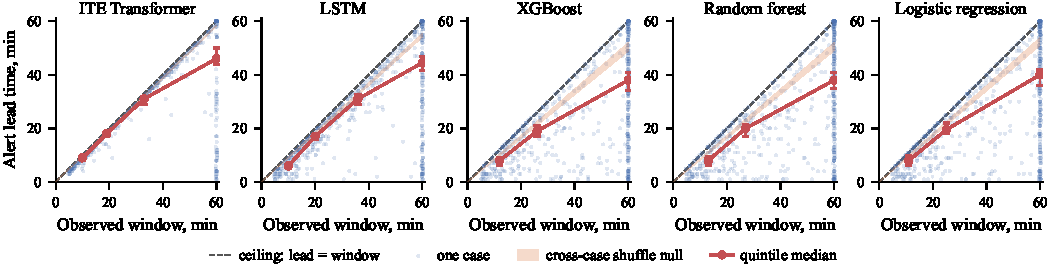
\includegraphics[width=\linewidth]{figures/Figure_A2_wide.pdf}
  \caption{\textbf{Alert lead time against observed window length, five model families, MOVER (EPIC) test.} Axes and overlays as in Figure 1. The relationship holds in every family; the transformer is the limiting case rather than the exception.}
  \label{fig:A1}
\end{figure}

\subsection{Alert composition}\label{alert-composition}

Section 5.1 reports the prevalent share as a single number per cell. For the transformer that
share is 8.7, 9.6 and 9.0\% in the three cohorts, and removing those cases moves its median lead
from 24, 17 and 22 minutes to 21, 15 and 19. Splitting detected event cases by when their first
crossing fell separates alerts that were already active at the first eligible minute from those
raised while the score was still settling and those raised later, which is the disclosure
Section 6.2's first item asks for.

\textbf{That share and Table A10's \texttt{Alerted\ by\ elapsed\ min\ 1} are different quantities rather than two
estimates of one.} The prevalent share counts detected event cases whose first crossing falls at
elapsed minute zero, the first minute of the case's own alert window, over the detected event
cases of that cell: 53 of 611, 66 of 684 and 83 of 926 for the transformer. Table A10's column
counts event cases whose first crossing falls at elapsed minute zero \textbf{or} minute one, over
every event case with a positive observed window, detected or not, as one minus the Kaplan-Meier
survival of time to first alert with each case censored at the end of its own window: 418 of 786,
463 of 1,007 and 434 of 1,409. Numerator, denominator and conditioning set all differ, and the
extra minute is the larger of the differences: minute one alone adds 365, 397 and 351 cases,
which is Section 4.1's settling read on the elapsed axis and not a second estimate of the same
immediate-alert probability. No case is censored before elapsed minute one in any of the three
cohorts, so the survival estimate at that mark equals the crude share.

\begin{figure}[H]
  \centering
  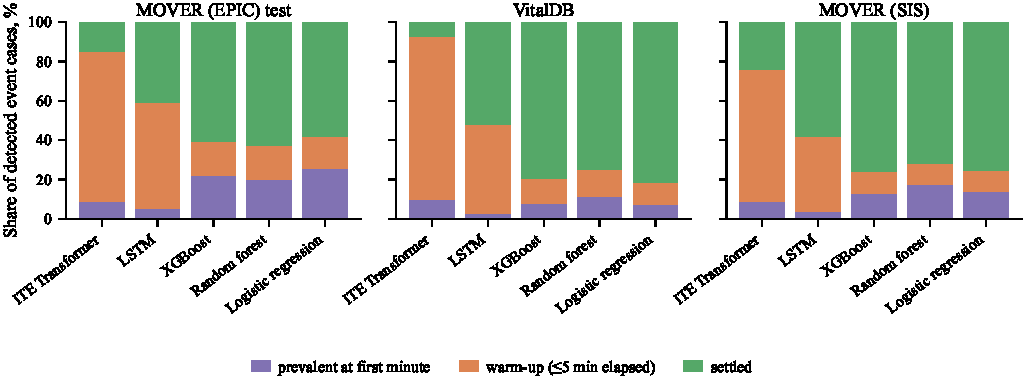
\includegraphics[width=\linewidth]{figures/Figure_3_wide.pdf}
  \caption{\textbf{Composition of detected event cases by elapsed monitoring time at the first crossing.} Prevalent cases are above threshold at their first eligible minute; warm-up cases cross within five minutes of it; settled cases cross later. Five model families, three cohorts, at the transported 80\%-sensitivity operating point. The composition differs sharply across families, in that the transformer's alerts are concentrated in the first five minutes, the LSTM's are partly so and the tabular families' are not, while the lead-to-window relationship of Section 3 holds in all of them. That is why Section 4 separates the transformer's direct mechanism from the cross-family directedness result.}
  \label{fig:A2}
\end{figure}

\subsection{Risk-set composition, and what fixing the cohort does}\label{risk-set-composition-and-what-fixing-the-cohort-does}

The population trajectory scores every case that has a minute in the bin, so its denominator
shrinks and its composition shifts as the bin moves away from onset. For an event case the
observable run-up \emph{is} its time to onset, so a short run-up is not missing data. It is an
early-onset event, and the far bins keep only the long run-ups. That is the same selection
that drives Section 3.

\textbf{Fixing the cohort moves the trajectory in both directions} (Figure A3). Recomputing the
same bins on the cases observable back to 60 minutes raises the far end and lowers the near
end, and the two curves cross at 16.4, 12.6 and 14.9 minutes before onset. The first bin
reaching AUROC 0.70 moves from 15 minutes in all three cohorts to 20, 35 and 20. Neither
curve is the true one: which denominator is used is a reporting choice, it changes the
horizon a reader would quote by up to twenty minutes, and it is not currently disclosed.
That is the whole of Section 6.2's third item.

\textbf{Short and long run-ups are different operations, which is why Section 5.3 calls this censoring
non-independent.} Splitting event cases at a 40-minute observable run-up, the long group's
operations are longer in every cohort, by a standardized mean difference of 0.394, 0.515 and
0.428, the largest imbalance on the list in all three; procedure group and ASA class are also
imbalanced beyond 0.1 in each. So a case with a short run-up is not a briefly watched version of
a case with a long one.

\begin{figure}[H]
  \centering
  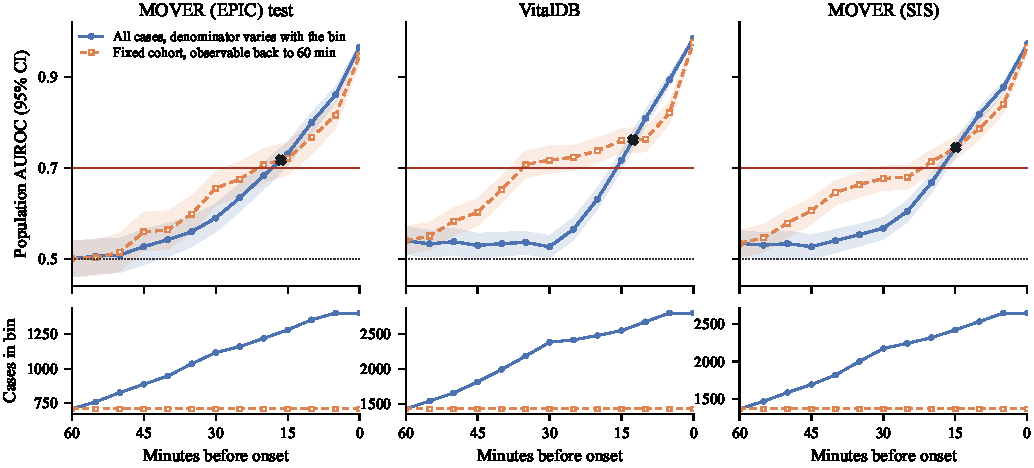
\includegraphics[width=\linewidth]{figures/Figure_A3_wide.pdf}
  \caption{\textbf{Population AUROC with its own risk set, event-aligned.} ITE Transformer, 2-minute bins from 60 minutes before onset to onset, in three held-out cohorts. Solid and filled is every case with a minute in the bin, the convention in the published literature, whose denominator varies; dashed and open is the cohort fixed to cases observable back to 60 minutes. Bands are 95\% cluster bootstrap over subjects, or over cases in MOVER (SIS). The lower row is the number of cases contributing to each bin, on its own scale per cohort. The dotted line marks 0.5, the solid rule 0.70, and the cross marks where the two curves meet.}
  \label{fig:A3}
\end{figure}

\subsection{Event and control score on the event-aligned axis}\label{event-and-control-score-on-the-event-aligned-axis}

The shape a reader expects of a continuously read score, rising in the cases that go on to
have an event and much flatter in the rest, is \textbf{present in all fifteen cells} (Figure A4).
Three things about it are worth reporting, and none is visible in a trend statistic.

\textbf{When the separation arrives runs opposite to near-onset discrimination.} For the three
tabular families the event and control means are already distinguishable 60 minutes before
onset in every cohort, the gap at that range running +0.049 to +0.109 with each pointwise
interval excluding zero. For the transformer the gap at 60 minutes \textbf{covers zero in all three
cohorts} ($-$0.023 {[}$-$0.080, 0.035{]}, $-$0.014 {[}$-$0.057, 0.030{]} and $-$0.006 {[}$-$0.043, 0.032{]}), and
first excludes it at 35, 20 and 30 minutes. The LSTM sits between the two. The family whose
scores separate latest is the one with the highest discrimination near onset.

\textbf{The event mean rises toward onset, and for the transformer the control mean falls by as
much.} Over the hour the transformer's event mean rises +0.239, +0.266 and +0.269, which is
the tendency a reader expects and it is substantial, while its control mean falls $-$0.252,
$-$0.263 and $-$0.196, so about half of the widening is carried by the controls. The LSTM's
control mean also falls, by 0.059 to 0.185. For the tabular families the control mean moves
between $-$0.070 and +0.021, rising in several cells, and the widening is almost entirely
event-side. So ``the score rises in patients who are about to have an event'' holds in every
cell here; what it leaves out is that for the transformer an equal share of the widening is
the control mean coming down, and an event-only trend statistic cannot separate the two.

\textbf{The split follows the representation more than the architecture.} The control side
contributes most where the window is read as a sequence and least where the model reads one
feature vector per scored minute, carrying each channel's last observation forward, so it sees
a level and has little shape to drift with. The ordering is not clean: the tabular families'
control means fall in MOVER (EPIC) as well and only flatten in the two external cohorts.
Representation and family are not crossed in this design, so this is a reading the data
supports rather than a hypothesis it tests. It does say where to look: \textbf{the control-side contribution is a thing
to measure in models given freer access to the input series}, and reporting the two sides of
a widening gap separately is what makes it visible.

Three things this figure is not. The control series is aligned on the sampled pseudo-onset of
Section 2 rather than on an event, so its fall is behavior over the last hour of a comparable
window and not an approach to anything. Figure A5 plots medians and this figure means, and the
two are not interchangeable here. And the two figures use different alignments: Figure A5's
axis is elapsed time from the case's first scored minute and covers the first ten minutes of
the record, where the transformer has just settled above its own 0.894 threshold, whereas the bins here
sit far later in the case, where its event mean is 0.383. \textbf{The two are not in conflict, and
the length of the plateau is what reconciles them.} The median score holds at or above the
transported threshold through elapsed minute 24, 21 and 17 in event cases and 23, 20 and 16
in controls, then falls to 0.03 to 0.31 by minute 30. Figure A5 covers the first ten of those
minutes and stops inside the plateau; every bin in this figure falls after it in all but the
shortest records.

\begin{figure}[H]
  \centering
  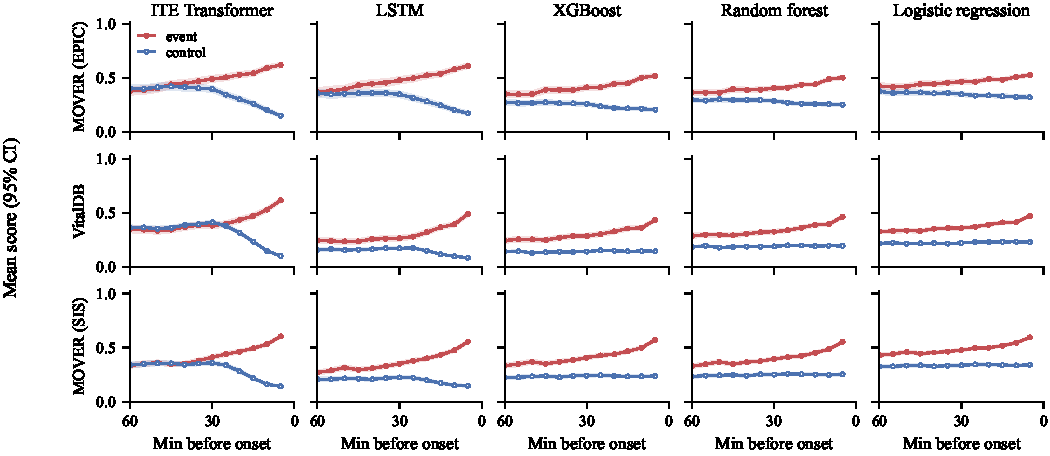
\includegraphics[width=\linewidth]{figures/Figure_A4_wide.pdf}
  \caption{\textbf{Mean score in event and control cases against minutes before onset.} Rows are cohorts, columns are model families, the same grid as Figure A5, on the event-aligned axis instead of the elapsed one. Event cases solid and filled, control cases dashed and open; bands are 95\% cluster bootstrap. Bins are the 13 centers at five-minute spacing from 60 minutes before onset; the bin at onset is empty by construction, because no minute is strictly before its own reference time, so the series ends at 5 minutes. Control cases are aligned on a sampled pseudo-onset.}
  \label{fig:A4}
\end{figure}

\subsection{Score against elapsed monitoring time}\label{score-against-elapsed-monitoring-time}

Section 4.1 reads the first ten monitored minutes of every case, and reports that the ITE
Transformer clears its own threshold there in every cohort. The margins for the others are wide.
Over those ten minutes the highest median score reached in either group is 0.69 against a
threshold of 0.78 for logistic regression in MOVER (EPIC), 0.65 against a threshold of 0.91 for
XGBoost, and 0.54 against a threshold of 0.79 for random forest. The LSTM is the one exception:
in MOVER (EPIC) it reaches 0.99 in event and 0.99 in control cases against a threshold of 0.97,
clearing it in both groups, and it clears it in neither external cohort. This is that view for
all fifteen cells, on the elapsed axis rather than the event-aligned one of Figure A4.

\begin{figure}[H]
  \centering
  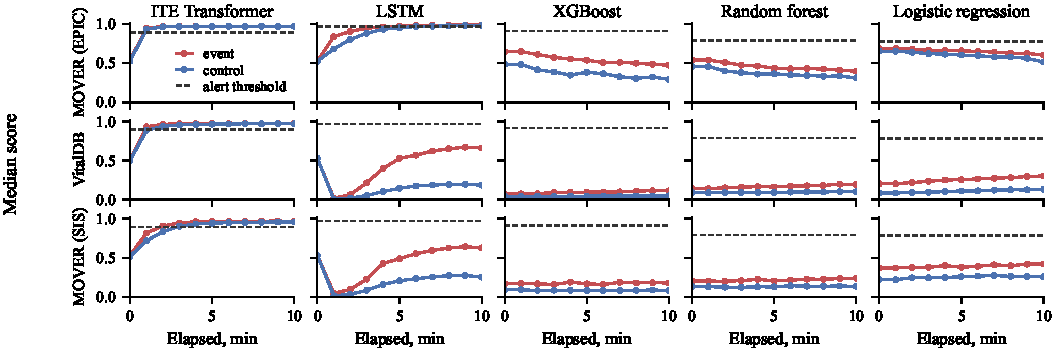
\includegraphics[width=\linewidth]{figures/Figure_1_wide.pdf}
  \caption{\textbf{Median score against elapsed monitoring time, with each family's own alert threshold.} Rows are cohorts, columns are model families. Elapsed time is measured from the case's first scored minute. The dashed rule in each panel is that family's transported raw-score threshold at the 80\%-sensitivity target, transferred unchanged from the MOVER (EPIC) validation split. Only the ITE Transformer's early rise clears its own threshold in every cohort, and it does so in event and control cases together; the LSTM does the same in MOVER (EPIC) alone. The elevation ends around minute 20, past the right edge of this axis. This axis is elapsed time; the event-aligned view is Figure A4.}
  \label{fig:A5}
\end{figure}

\subsection{Departure timing: searched for, not found}\label{departure-timing-searched-for-not-found}

We asked whether the score departs from its own baseline before mean arterial pressure
departs from its, within an episode, under a pre-specified rule: baseline is the median of
the episode's first ten eligible minutes, the robust scale is 1.4826 $\times$ the median absolute
deviation over the same minutes, and a departure is the first minute beginning a run of at
least three consecutive minutes more than 1.5 scale units in the deteriorating direction.

\textbf{Score departure does not precede MAP departure.} For XGBoost the share of episodes in
which the score departs first is significantly \emph{below} one half in all three cohorts. For the
transformer the score does not depart at all in most episodes, because its baseline sits at the
top of its range: a median baseline of 0.94 to 0.97 leaves median headroom of 0.005 to 0.031,
which is less than the bar its own rule sets in all three cohorts, so there is not enough room
above baseline for a departure to register.
Both facts are reported so the negative cannot be read as an unfair rule. Sensitivity
analyses at a 2.0 scale threshold, a five-minute run length, and a search capped at the
60-minute window all leave the direction unchanged.

The question was pre-specified and the answer constrains Section 4: whatever produces the
reported lead, it is not the score moving before the monitored variable does.

\subsection{Lead time by band, the transformer's three cohorts}\label{lead-time-by-band-the-transformers-three-cohorts}

\begin{minipage}{\linewidth}
\textbf{Table A9 \textbar{} Median alert lead time inside quantile-derived bands of observed window, ITE Transformer.} ITE
Transformer, three held-out cohorts, at the transported 80\%-sensitivity operating point.
Quintile edges are cut within each cell on detected cases; where the observed window is censored
at the 60-minute alert window the upper quintiles collapse and the realized band count is
reported rather than assumed. \texttt{Observed\ window,\ min} is the median observed pre-onset window of that band's cases rather than
an edge. Intervals are 95\% cluster bootstrap over subjects, or over cases in MOVER (SIS). All fifteen cells are Table A1; the detection rate these bands condition on is Table A5.
Section 3.1 reports the contrast this table carries.

\vspace{0.5em}
\centering\footnotesize
\begin{tabular}{@{}lrrrll@{}}
\toprule
Cohort & Band & n & Observed window, min & Median lead, min (95\% CI) & Lead / window (95\% CI) \\
\midrule
MOVER (EPIC) test & 1 & 139 & 10 & 9 {[}8, 9{]} & 0.88 {[}0.85, 0.89{]} \\
MOVER (EPIC) test & 2 & 111 & 19 & 18 {[}17, 18{]} & 0.94 {[}0.94, 0.95{]} \\
MOVER (EPIC) test & 3 & 121 & 33 & 31 {[}29, 32{]} & 0.97 {[}0.96, 0.97{]} \\
MOVER (EPIC) test & 4 & 240 & 60 & 46 {[}44, 50{]} & 0.98 {[}0.96, 0.98{]} \\
VitalDB & 1 & 143 & 7 & 5 {[}5, 6{]} & 0.83 {[}0.83, 0.83{]} \\
VitalDB & 2 & 140 & 12 & 10 {[}10, 11{]} & 0.91 {[}0.90, 0.91{]} \\
VitalDB & 3 & 132 & 20 & 19 {[}18, 20{]} & 0.94 {[}0.94, 0.95{]} \\
VitalDB & 4 & 134 & 40 & 38 {[}37, 40{]} & 0.97 {[}0.97, 0.97{]} \\
VitalDB & 5 & 135 & 60 & 59 {[}57, 60{]} & 0.98 {[}0.98, 1.00{]} \\
MOVER (SIS) & 1 & 199 & 8 & 6 {[}5, 6{]} & 0.80 {[}0.80, 0.82{]} \\
MOVER (SIS) & 2 & 179 & 17 & 14 {[}13, 15{]} & 0.86 {[}0.84, 0.91{]} \\
MOVER (SIS) & 3 & 186 & 29 & 27 {[}26, 28{]} & 0.94 {[}0.93, 0.96{]} \\
MOVER (SIS) & 4 & 362 & 60 & 46 {[}43, 49{]} & 0.95 {[}0.93, 0.97{]} \\
\bottomrule
\end{tabular}
\end{minipage}

\vspace{0.8em}

\subsection{Cohort composition and the control side}\label{cohort-composition-and-the-control-side}

\begin{minipage}{\linewidth}
\textbf{Table A10 \textbar{} Cohort composition, PPV against prevalence, and the control side.} \texttt{PPV\ $-$\ prevalence} is the lift over the base rate of the cohort the PPV is measured in, because raw PPV
is not comparable across cohorts whose prevalence runs from 0.359 to 0.560. \texttt{Alerted\ by\ elapsed\ min\ 1} is one minus the Kaplan-Meier survival of time to first alert at the first elapsed
monitoring minute, censored at the end of each case's own window; it is the censoring-aware form
of Section 4.1's settling. It is \textbf{not} the prevalent share of Section 5.1, which uses a
different numerator and a different denominator; Appendix A.11 sets the two estimands out side by
side. Intervals are 95\% cluster bootstrap.

\vspace{0.5em}
\centering\footnotesize
\begin{tabular}{@{}
  >{\raggedright\arraybackslash}p{(\columnwidth - 14\tabcolsep) * \real{0.140}}
  >{\raggedright\arraybackslash}p{(\columnwidth - 14\tabcolsep) * \real{0.110}}
  >{\raggedleft\arraybackslash}p{(\columnwidth - 14\tabcolsep) * \real{0.125}}
  >{\raggedleft\arraybackslash}p{(\columnwidth - 14\tabcolsep) * \real{0.125}}
  >{\raggedleft\arraybackslash}p{(\columnwidth - 14\tabcolsep) * \real{0.140}}
  >{\raggedleft\arraybackslash}p{(\columnwidth - 14\tabcolsep) * \real{0.140}}
  >{\raggedright\arraybackslash}p{(\columnwidth - 14\tabcolsep) * \real{0.110}}
  >{\raggedright\arraybackslash}p{(\columnwidth - 14\tabcolsep) * \real{0.110}}@{}}
\toprule
Model & Cohort & Event cases & Control cases & Prevalence & PPV $-$ prevalence & Min. above thr., controls (95\% CI) & Alerted by elapsed min 1 (95\% CI) \\
\midrule
ITE Transformer & MOVER (EPIC) test & 786 & 618 & 0.560 & +0.065 & 0.150 {[}0.050, 0.233{]} & 0.532 {[}0.497, 0.565{]} \\
ITE Transformer & VitalDB & 1007 & 1797 & 0.359 & +0.021 & 0.183 {[}0.163, 0.233{]} & 0.460 {[}0.428, 0.491{]} \\
ITE Transformer & MOVER (SIS) & 1409 & 1232 & 0.534 & +0.051 & 0.025 {[}0.017, 0.047{]} & 0.308 {[}0.285, 0.332{]} \\
LSTM & MOVER (EPIC) test & 786 & 618 & 0.560 & +0.101 & 0.017 {[}0.000, 0.027{]} & 0.228 {[}0.198, 0.257{]} \\
LSTM & VitalDB & 1007 & 1797 & 0.359 & +0.236 & 0.000 {[}0.000, 0.000{]} & 0.087 {[}0.071, 0.105{]} \\
LSTM & MOVER (SIS) & 1409 & 1232 & 0.534 & +0.151 & 0.000 {[}0.000, 0.000{]} & 0.138 {[}0.120, 0.157{]} \\
XGBoost & MOVER (EPIC) test & 786 & 618 & 0.560 & +0.165 & 0.000 {[}0.000, 0.000{]} & 0.188 {[}0.161, 0.215{]} \\
XGBoost & VitalDB & 1007 & 1797 & 0.359 & +0.253 & 0.000 {[}0.000, 0.000{]} & 0.062 {[}0.047, 0.077{]} \\
XGBoost & MOVER (SIS) & 1409 & 1232 & 0.534 & +0.180 & 0.000 {[}0.000, 0.000{]} & 0.119 {[}0.101, 0.136{]} \\
Random forest & MOVER (EPIC) test & 786 & 618 & 0.560 & +0.143 & 0.000 {[}0.000, 0.000{]} & 0.183 {[}0.157, 0.212{]} \\
Random forest & VitalDB & 1007 & 1797 & 0.359 & +0.221 & 0.000 {[}0.000, 0.000{]} & 0.101 {[}0.082, 0.121{]} \\
Random forest & MOVER (SIS) & 1409 & 1232 & 0.534 & +0.154 & 0.000 {[}0.000, 0.000{]} & 0.166 {[}0.147, 0.186{]} \\
Logistic regression & MOVER (EPIC) test & 786 & 618 & 0.560 & +0.128 & 0.000 {[}0.000, 0.017{]} & 0.226 {[}0.198, 0.255{]} \\
Logistic regression & VitalDB & 1007 & 1797 & 0.359 & +0.237 & 0.000 {[}0.000, 0.000{]} & 0.036 {[}0.025, 0.048{]} \\
Logistic regression & MOVER (SIS) & 1409 & 1232 & 0.534 & +0.152 & 0.000 {[}0.000, 0.000{]} & 0.121 {[}0.104, 0.138{]} \\
\bottomrule
\end{tabular}
\end{minipage}

\vspace{0.8em}

\subsection{What the label invites, and what the number supports}\label{what-the-label-invites-and-what-the-number-supports}

\begin{minipage}{\linewidth}
\textbf{Table A11 \textbar{} What the label invites, and what the number supports.} Column one is an affordance
of the reported label in the sense Section 1 defines, not measured comprehension. Column two is what this paper's
measurement supports in its place, and column three the disclosure that would separate them.

\vspace{0.5em}
\centering\footnotesize
\begin{tabular}{@{}
  >{\raggedright\arraybackslash}p{(\columnwidth - 4\tabcolsep) * \real{0.21}}
  >{\raggedright\arraybackslash}p{(\columnwidth - 4\tabcolsep) * \real{0.45}}
  >{\raggedright\arraybackslash}p{(\columnwidth - 4\tabcolsep) * \real{0.34}}@{}}
\toprule
What the label invites & What the number supports here & The disclosure that would close the gap \\
\midrule
The model warns about 24 minutes ahead & A median over detected event cases, itself a window-dependent set, under this cohort's window distribution (Section 3.1) & The pre-onset window distribution, and a window-conditional timing statistic (Section 6.2) \\
Twenty-four minutes is a property of the model & Within one model and cohort, median lead rises across window bands by 26 to 54 minutes, in 15 of 15 cells (Table A1) & Any single median stratified by the realized available window (Section 6.2) \\
Twenty-four minutes of usable warning & A lead read at case-level specificity 0.406, the lowest of the five families in that cohort (Table A4) & The operating point reported beside the lead (Sections 4.1, 6.3) \\
A longer lead indicates a better model & A descriptive association running the other way: lead is opposite to specificity across the fifteen combinations, Spearman $-$0.803 (Section 4.1) & Lead and operating point reported together, not lead alone (Section 6.3) \\
\bottomrule
\end{tabular}
\end{minipage}

\vspace{0.8em}

\subsection{Multiplicity}\label{multiplicity}

The two nulls of Section 3.3 form one Benjamini--Hochberg family of 75 formal tests,
adjusted within that family, of which 57 are significant at \emph{q} \textless{} 0.05. The stratification of Section 3.1 produces intervals rather than tests and does not enter the family.
Every bootstrap interval in this paper, including the fifteen window-gradient intervals of
Table A1, is a \textbf{pointwise descriptive interval}: no family-wise coverage claim is made across
the fifteen contrasts, and ``each interval excludes zero'' is fifteen separate statements rather
than one simultaneous one.

\subsection{Seeds and reproducibility}\label{seeds-and-reproducibility}

Cluster bootstraps use 2,000 replicates, with the clustering unit the subject for two cohorts
and the case for MOVER (SIS), whose released subject key is a copy of the case identifier. The
two nulls of Section 3.3 draw 1,000 permutations per cell. The cross-combination rank
correlations of Section 4.1 are reported as \textbf{point estimates with no accompanying test}. A
permutation of the pairing was computed while this analysis was being developed, and is not
reported: its unit is a cell, and cells sharing a cohort or a model family are not
exchangeable, so the resulting \emph{P} value would overstate what fifteen dependent combinations
can establish. Section 4.1 gives the untied-pair counts and the within-cohort correlations in
its place. Model training and the reference-time construction are fixed at a single seed,
reported in Appendix A.1.
